\subsection{Typical \IOT Scenarios}
\label{sec:Motivation-Scenarios}

Figure \ref{fig:scenario} describes a typical configuration at Alice's smart home, the fictional character we use in our case study. Alice asked her technician to deploy light sensors and bulbs to lighten the rooms, motion and door detectors to detect human activity, an alarm used in case of emergency and a toggle button placed in the balcony for security purposes.

\begin{figure}%
	\centering  
	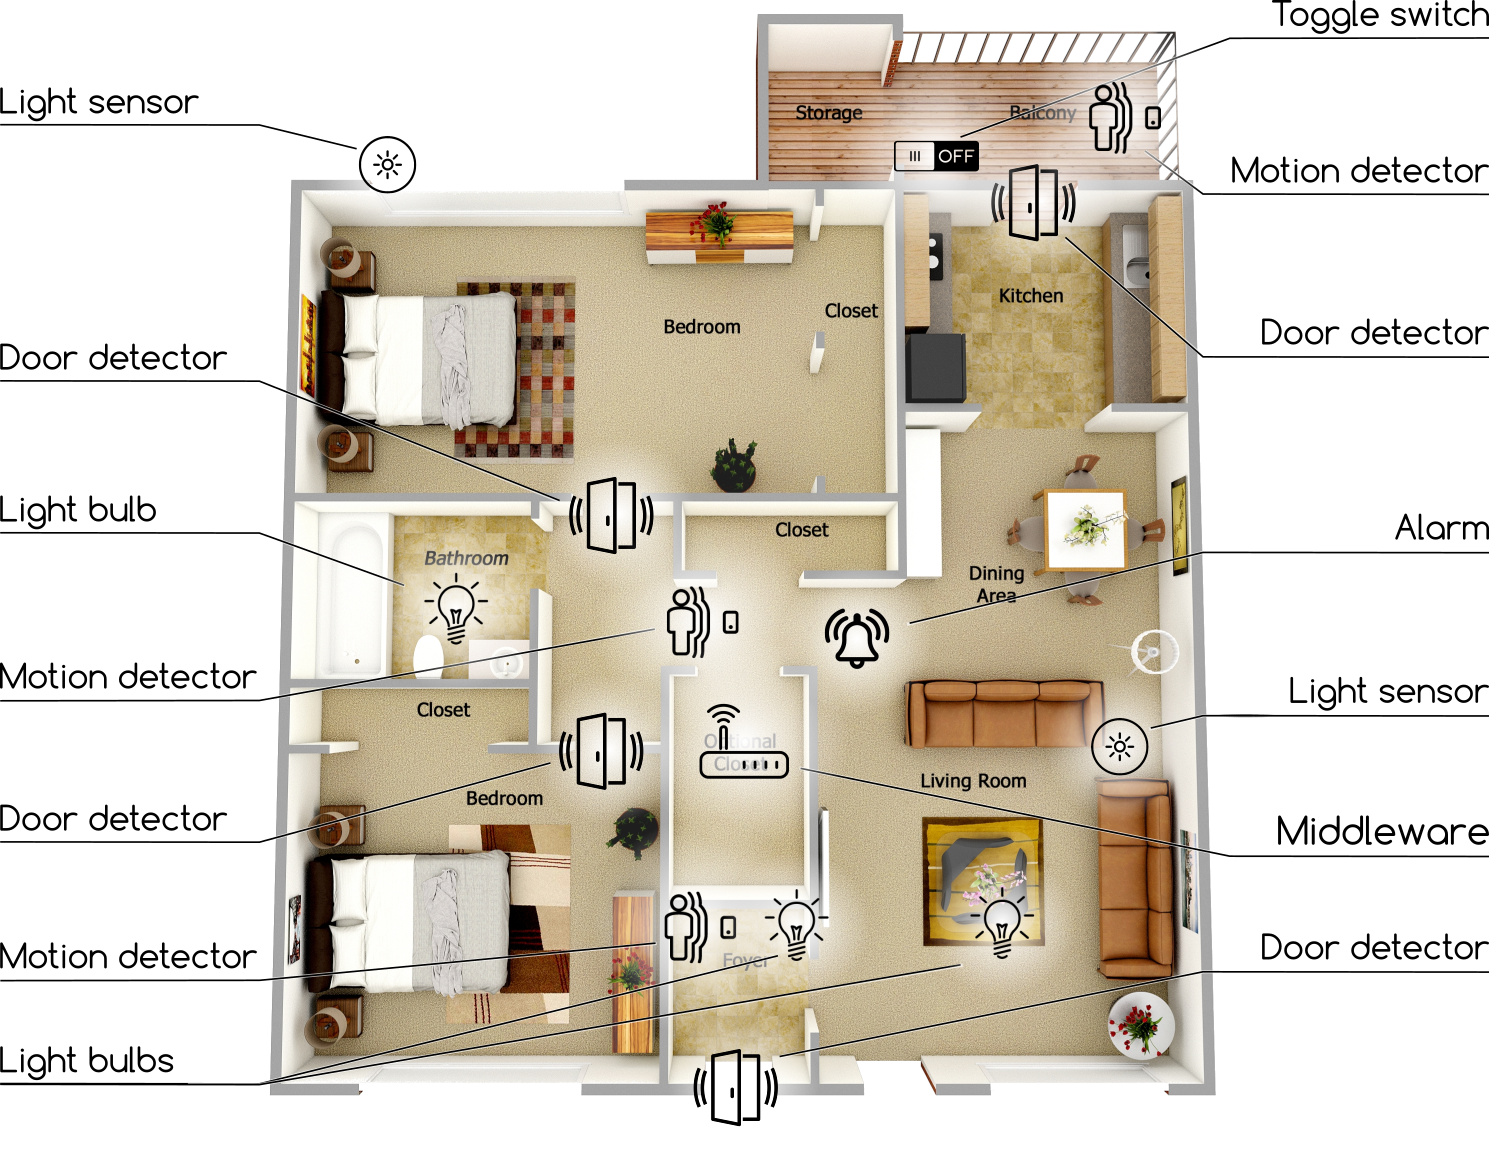
\includegraphics[width=.9\linewidth]{scenario.png}%
	\caption{Hypothetical Alice's \textit{smart-home} configuration of \IOT devices}%
	\label{fig:scenario}%
\end{figure}

Alice is interested in simple scenarios for her comfort and her little boy's security: she wants the entrance lights to automatically switch on to welcome her when she arrives home. Also since her boy often plays in the balcony, or sometimes wakes up at night and walks through the apartment, she needs to ensure he does not fall or injure himself. Those scenarios may be meet with her current equipment as we will illustrate in Section \ref{sec:IoTDSL-BusinessRules} with a set of rule-based specifications.
